\chapter{Discussion}\label{discussion}

The scheme is explicit about what the vector cannot do, for example: Material, thermal and hydrological identities do not follow from RES geometry. So where two physically different beds collapse onto one vector the scheme labels it degenerate rather than resolving it by assumption. 


\section{Data Representativeness and Model Utility}
% \begin{figure}
%     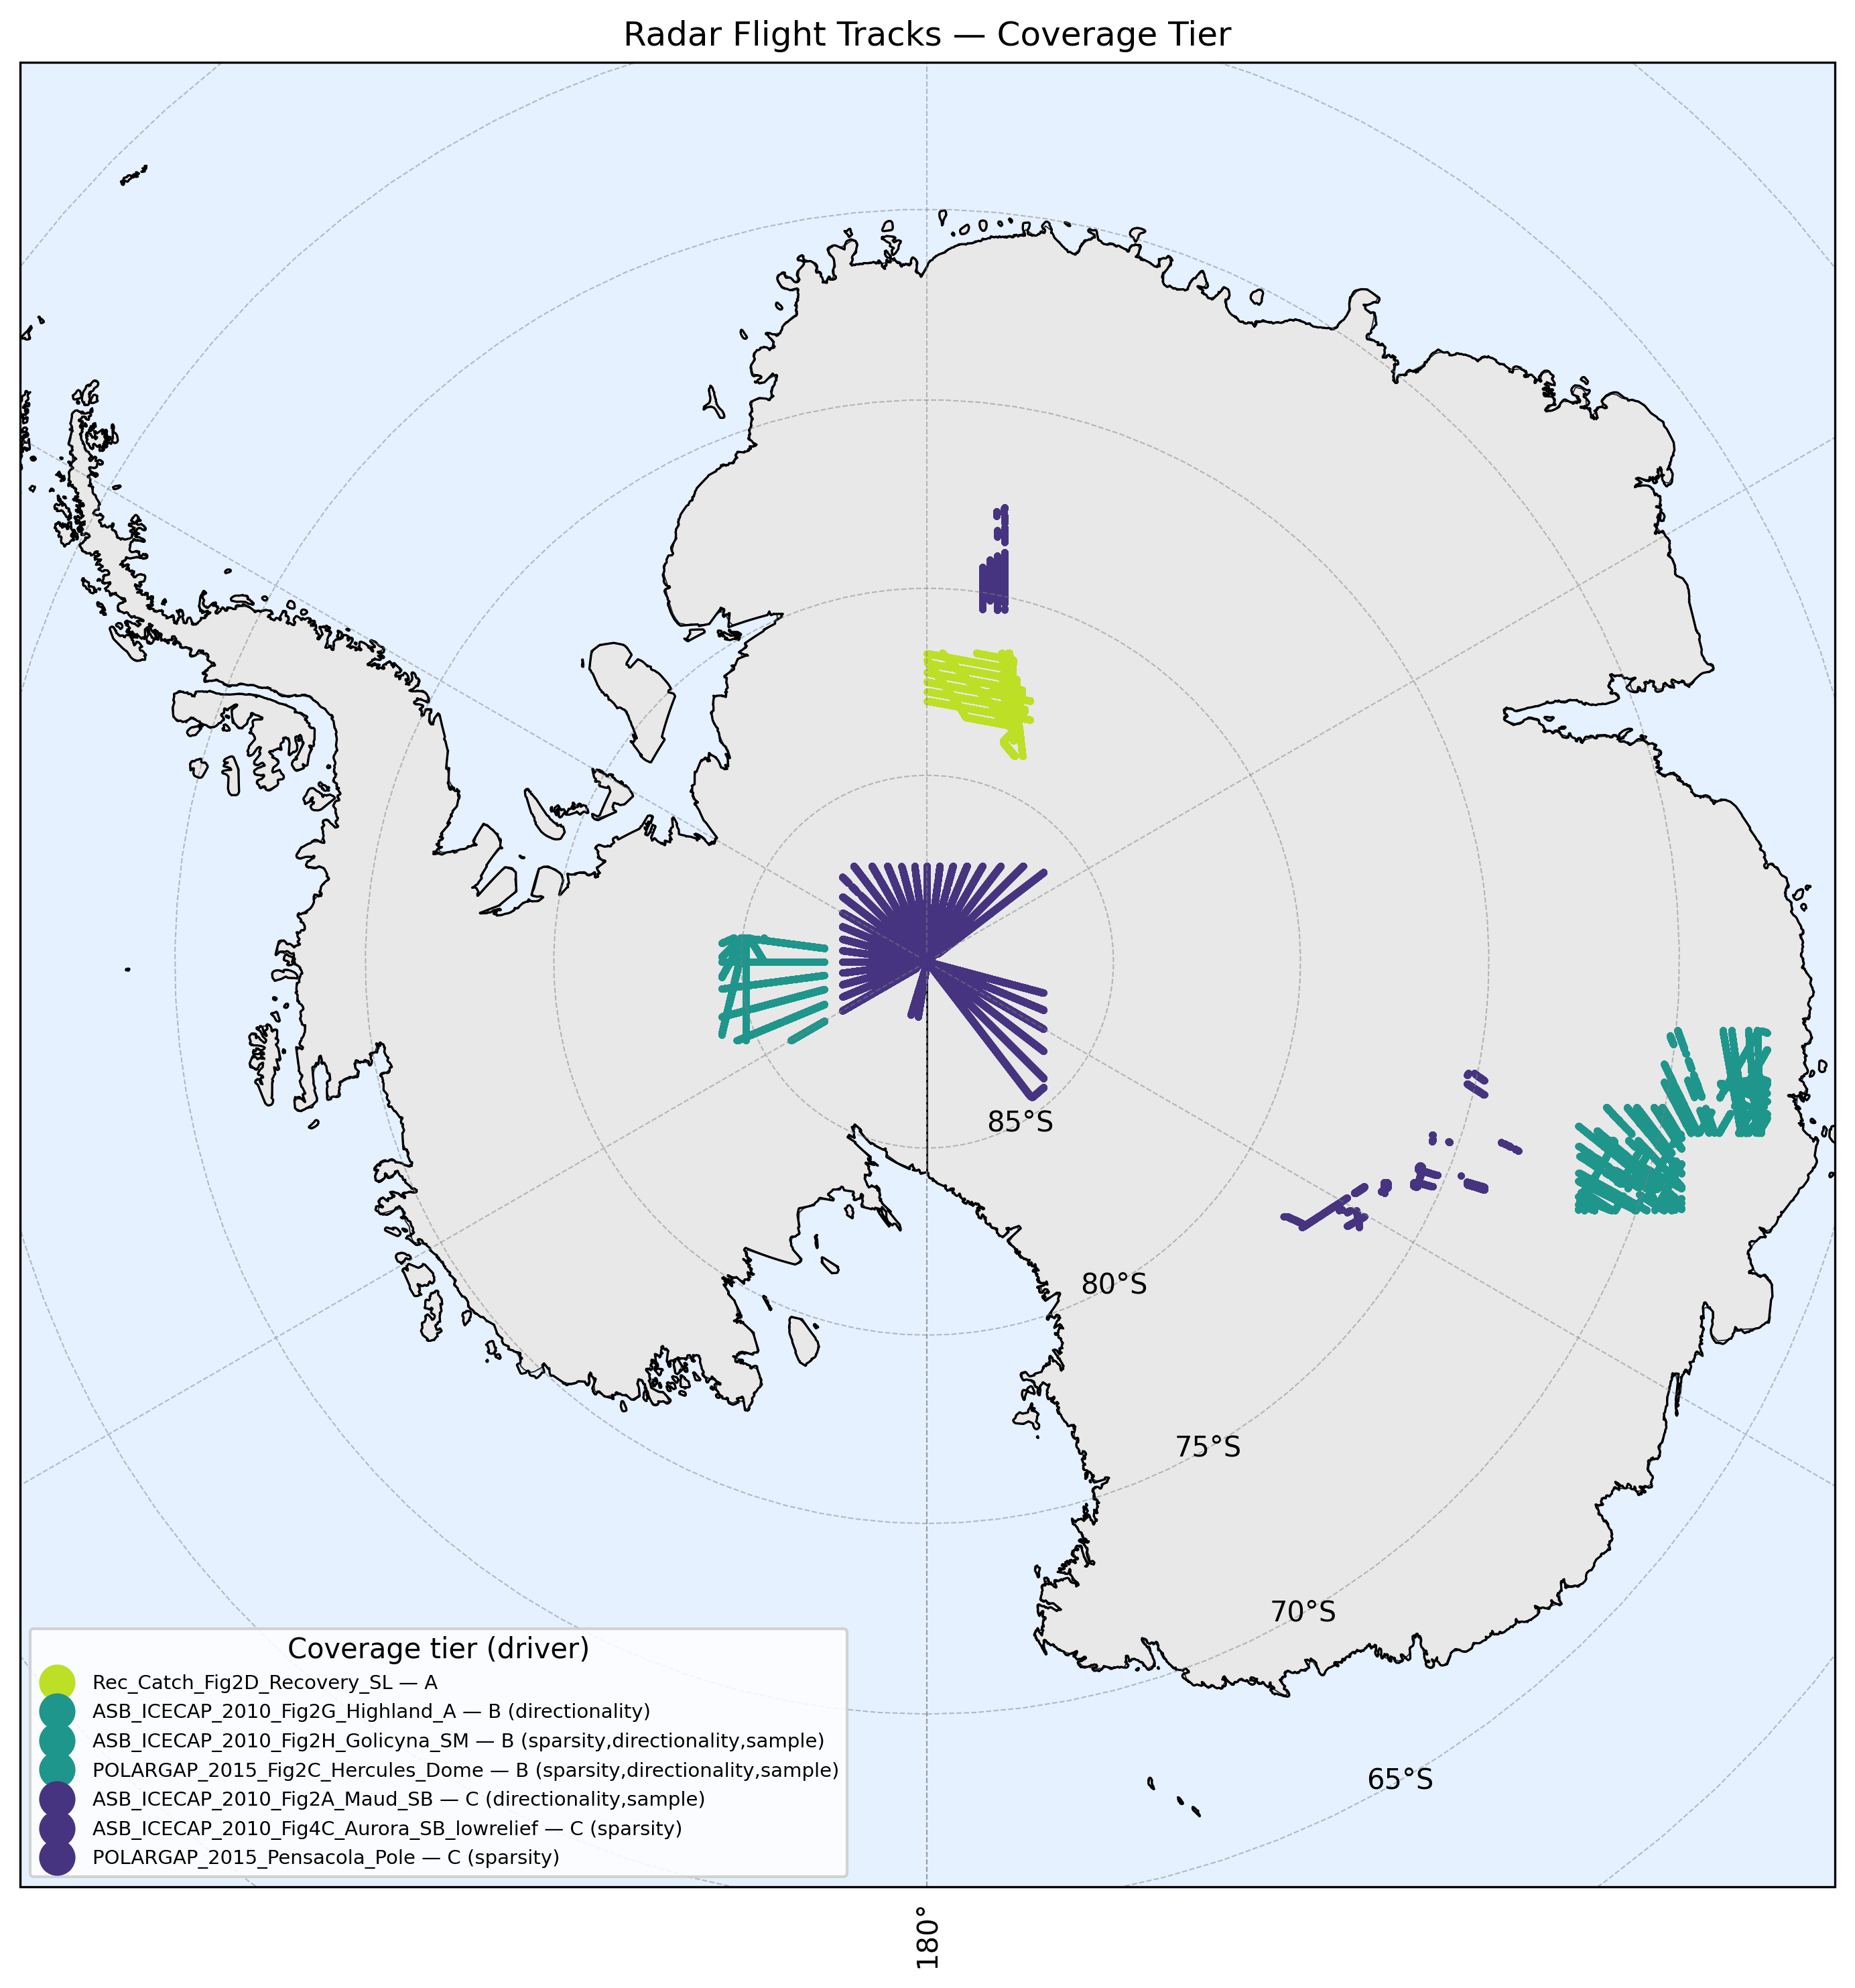
\includegraphics[scale=0.038]{figures/antarctica_tracks_tier.png}
%     \caption{% Full Antarctic overview showing flight line coverage tiers (\texttt{A/B/C}) based on sparsity (\texttt{gap\_p90}), directionality (\texttt{azimuth\_R}), and sample size (\texttt{n\_homog}).} 
%     \label{fig:coverage_tiers}
% \end{figure}

% \begin{figure}
%     \includegraphics[scale=0.038]{figures/????}
%     \caption{} 
%     \label{fig:model_utility}
% \end{figure}

\section{Ockenden landscapes comparison}

% \begin{figure}
%     \includegraphics[scale=0.37]{figures/????}
%     \caption{My own coloured map classification for comparison} 
%     \label{fig:7-regions_over_Ockenden}
% \end{figure}


% \begin{figure}
%     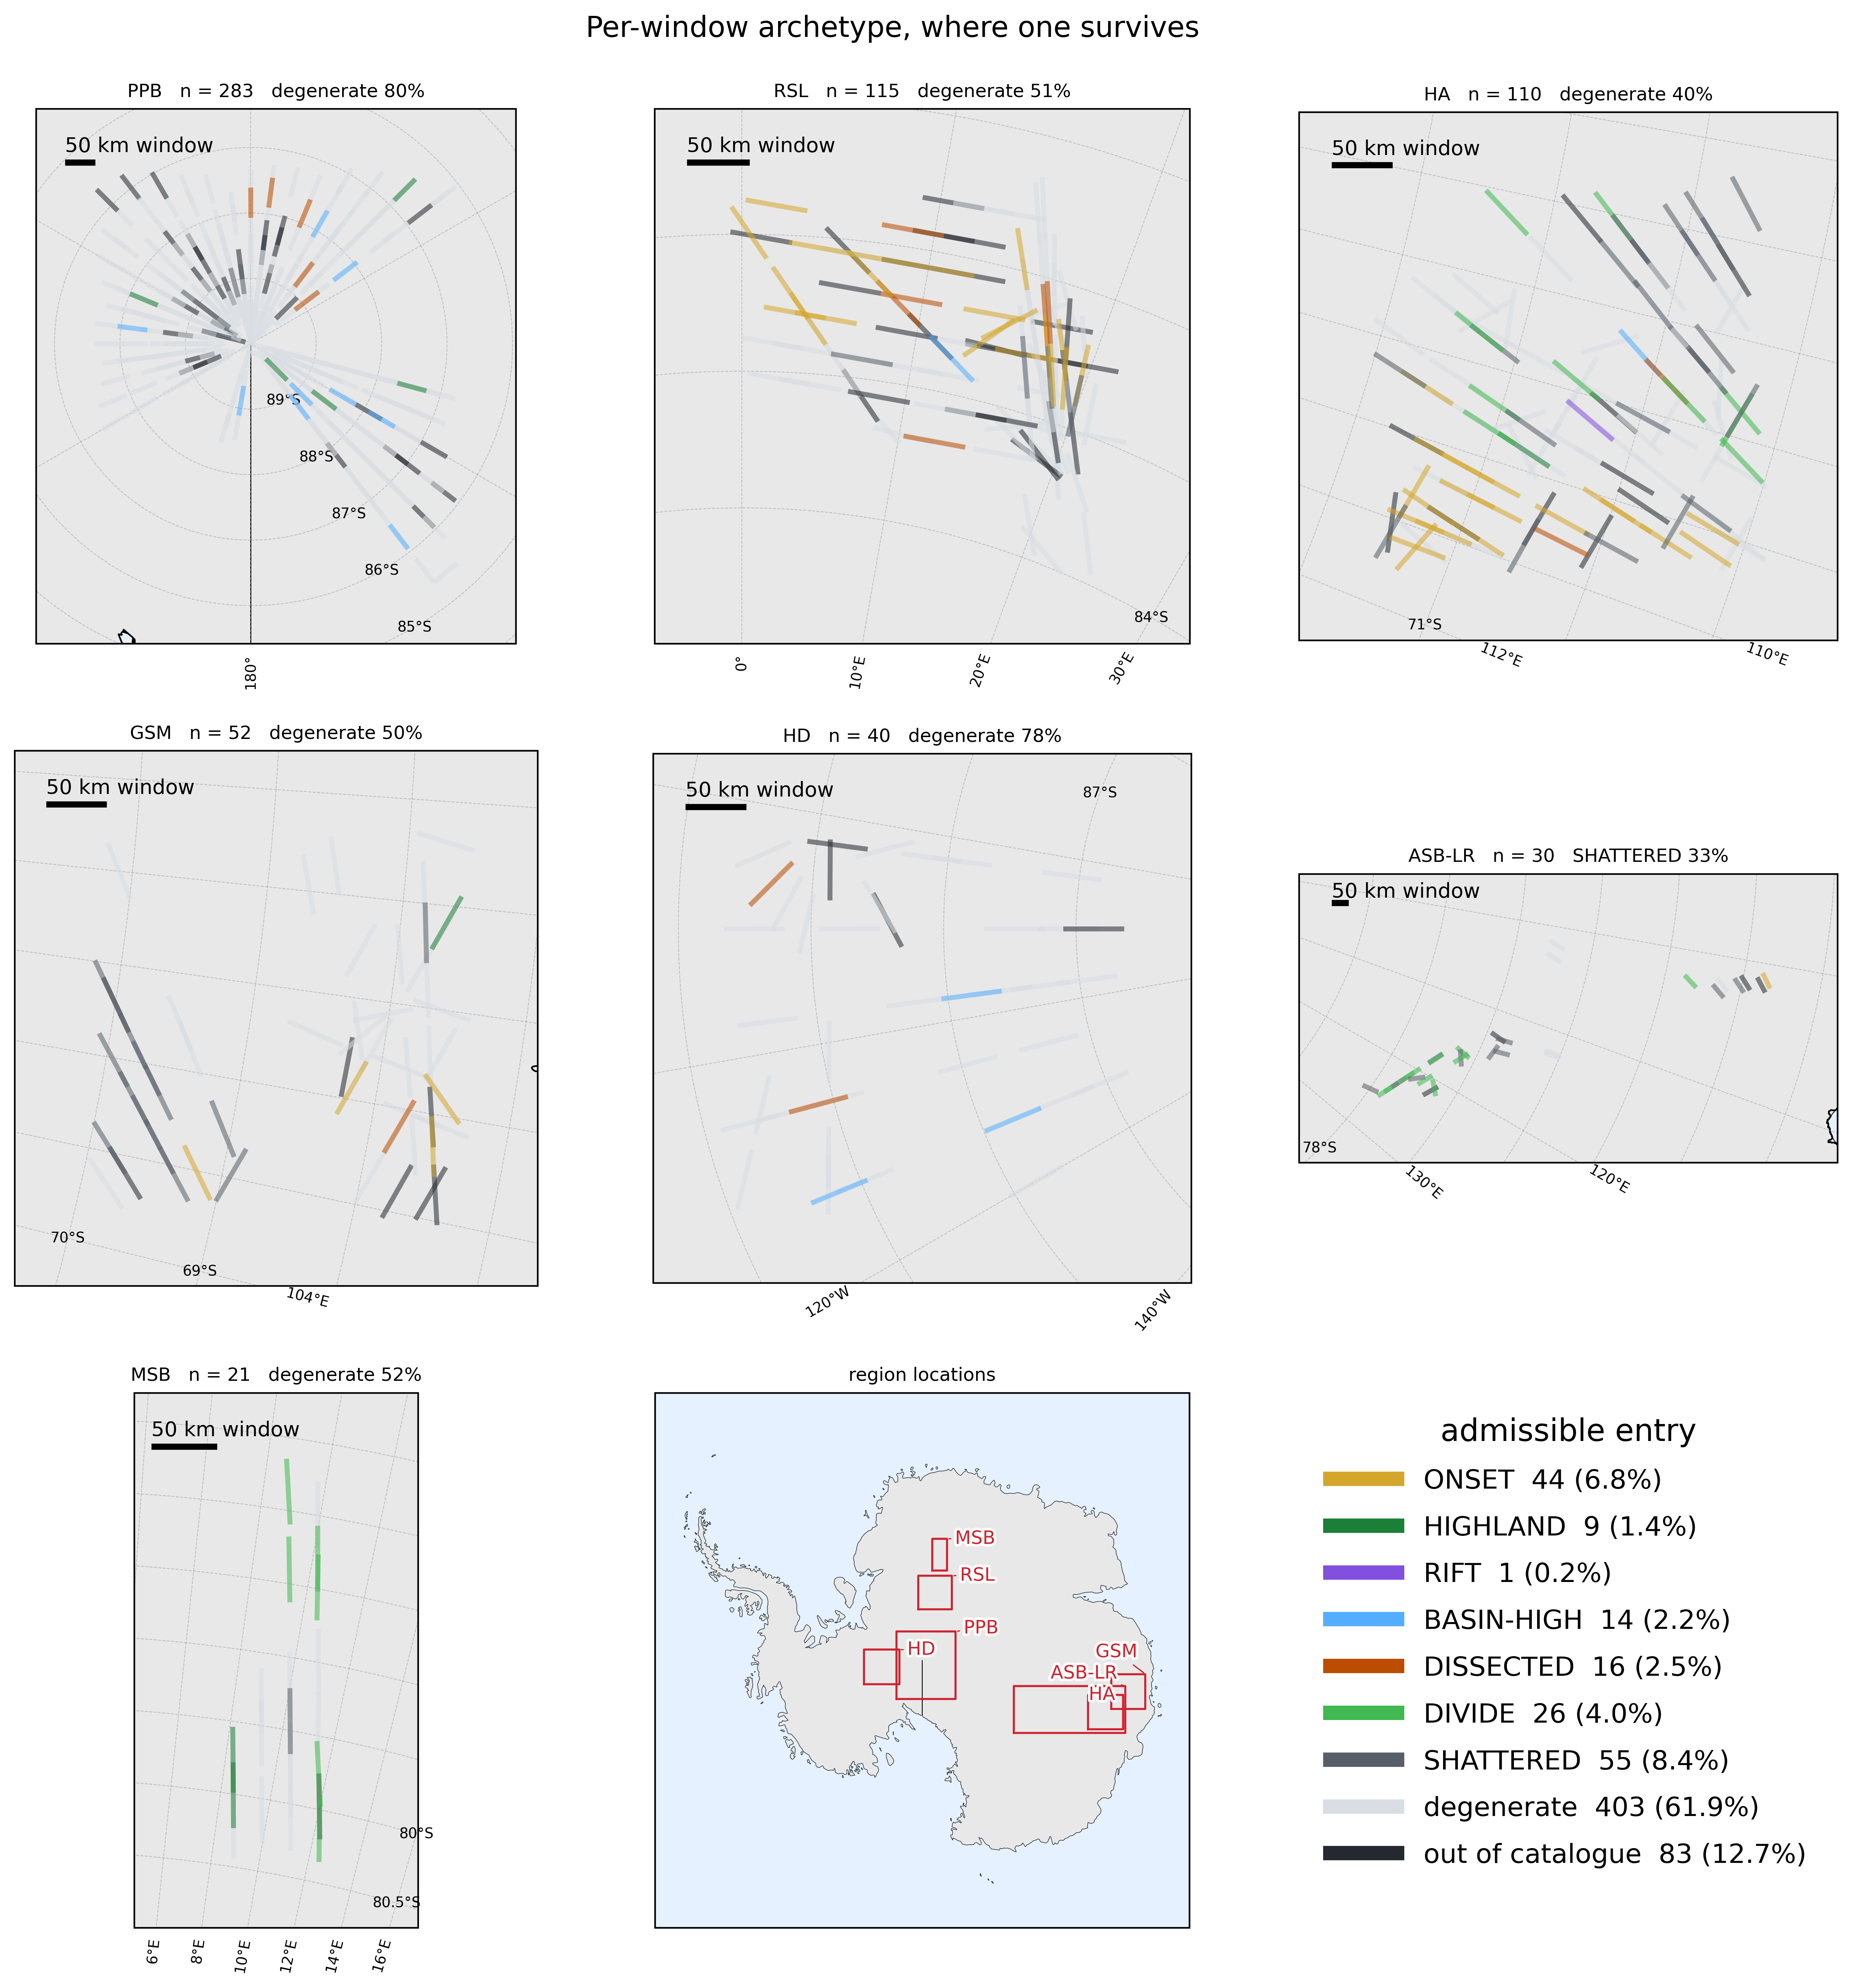
\includegraphics[scale=0.37]{figures/fig6b_archetype_map.png}
%     \caption{} 
%     \label{fig:archetype_map_windows}
% \end{figure}
